\documentclass[11pt,a4paper]{article}
\usepackage[T1]{fontenc}
\usepackage[utf8]{inputenc}
\usepackage{lmodern,amsmath,amssymb,booktabs,array,graphicx,geometry,natbib,microtype}
\usepackage{placeins}
\usepackage[hidelinks]{hyperref}
\usepackage{fancyhdr}
\geometry{margin=24mm}
\setlength{\headheight}{14pt}
\setlength{\parskip}{2pt}
\setlength{\parindent}{1.2em}
\setlength{\emergencystretch}{2em}
\graphicspath{{../figures/}}
\usepackage{caption}
\captionsetup{font=small,labelfont=bf}
\renewcommand{\topfraction}{0.9}
\renewcommand{\bottomfraction}{0.8}
\renewcommand{\textfraction}{0.08}
\renewcommand{\floatpagefraction}{0.72}
\setcounter{topnumber}{3}
\setcounter{bottomnumber}{2}
\setcounter{totalnumber}{5}
% Replace with the verified public record citation after deposit. No DOI is invented.
\newcommand{\AnalysisAvailability}{The tabulated results, figure data and supplementary diagnostics are supplied in the accompanying machine-readable analysis package. The fitting and resampling code and full numerical outputs can be obtained from the author.}

\pagestyle{fancy}\fancyhf{}
\fancyhead[L]{\small Mass loss and halo velocity structure}
\fancyhead[R]{}
\fancyfoot[C]{\thepage}
\newcommand{\doi}[1]{\href{https://doi.org/#1}{doi:\nolinkurl{#1}}}
\newcommand{\yv}{Y_v}
\newcommand{\Mrec}{M_{\mathrm{max,rec}}}
\newcommand{\Mterm}{M_{\mathrm{term}}}
\hypersetup{pdftitle={Mass-loss dependence of accretion-history correlations in dark-matter halo velocity structure},pdfauthor={Stephen Atalebe},pdfsubject={Continuous recorded-mass-loss control, population sensitivity and structural assembly-history information}}
\title{Mass-loss dependence of accretion-history correlations\\in dark-matter halo velocity structure}
\author{Stephen Atalebe\\\small Independent researcher}
\date{}
\begin{document}
\maketitle

\begin{abstract}
Recorded mass loss captures much of the fitted correlation between accretion history and halo velocity structure. We analyse mass-normalized maximum circular velocity in three TNG100-1-Dark and three BolshoiP samples, using different history operators and mass definitions. After terminal mass, current growth and four formation epochs are controlled, adding the logarithmic maximum-to-terminal mass ratio reduces the history-associated increments in explained variance by $51.6$--$92.7$ per cent across these separate analyses. An indicator-plus-quadratic loss model leaves increments of $0.0027$--$0.0112$ in mixed TNG, $0.0018$--$0.0131$ among TNG centrals and $0.0192$--$0.0205$ in baseline BolshoiP. All 30 linear- and flexible-loss fits have negative history coefficients. Conditional on unverified global residual exchangeability, design-specific permutations repeating the 26-value weighting search yield Holm-adjusted values of $0.030$ across 30 fiducial comparisons. TNG III centrals does not reject under single-step Bonferroni; no case rejects in the 60-comparison family including searched minima. A separate cubic-spline calculation gives consistent residual increments. After loss adjustment, coefficient-to-spatial-jackknife ratios are $2.10$--$4.22$ in TNG and $9.75$--$22.86$ in BolshoiP; the weakest TNG nominal $t$ comparisons approach $0.05$ and are not search-adjusted or spatially calibrated. Reweighting complete BolshoiP cases to available-sample mass-bin frequencies leaves similar increments, but does not recover missing formation epochs. Tidal evolution offers a physical comparison, not a calibration of the fitted coefficients. The results indicate substantial mass-loss dependence and a smaller population-dependent structural correlation within the tested models.
\end{abstract}
\noindent\textit{Key words:} dark matter -- galaxies: haloes -- cosmology: theory -- methods: numerical -- methods: statistical.

\section{Introduction}
The structure of a dark-matter halo records its gravitational assembly. The Navarro--Frenk--White profile provides a compact description of equilibrium halo structure, while the concentration--assembly relation connects internal density to mass growth \citep{NFW1997,Bullock2001,Wechsler2002}. The question addressed here is therefore more specific than whether assembly history matters: how much of a history-associated structural relation remains after a specified set of formation epochs and current properties has been included?

A formation epoch records a threshold crossing and discards most of the intervening trajectory. \citet{Zhao2009} relate concentration to the time when a main progenitor attained 4 per cent of its mass at the epoch of interest. \citet{Ludlow2013} connect the main-progenitor mass-accretion history to the present mass profile and its characteristic density. Their later collapsed-mass-history formulation considers the total mass in progenitors rather than only the main ancestor \citep{Ludlow2016}. These results motivate explicit comparisons between historical representations. Concentration models also incorporate peak height, power-spectrum shape and the evolution of halo boundaries \citep{DiemerJoyce2019}, while profile decompositions distinguish orbiting matter from current infall \citep{Diemer2023}. These are related descriptions of halo structure, rather than direct tests of the scalar residual examined here.

Other features of assembly contribute to structural variation. Principal-component analyses separate overall assembly age from late growth \citep{Wong2012}. Merger events produce lasting changes in concentration and contribute to its scatter at fixed mass and formation time \citep{Wang2020}. Machine-learning analyses connect different parts of the mass profile to different assembly times and recover low-dimensional representations involving early assembly and recent accretion \citep{LS2022,LS2024}. Our scalar-response regression is a simpler test of historical compression than those profile-level analyses.

We use \emph{residual accretion-history correlation} to denote the association of a compressed mass-growth history with halo structure after the stated controls. The term refers to a reduced statistical description. A dynamical claim would additionally require a future target, a specified evolving state and a test of whether the past improves that evolution model after conditioning on the available present state. Here the measured response is contemporaneous structure.

Our main empirical result is that the continuous maximum-to-terminal mass contrast captures a large part of the weighted-history association on identical populations; a smaller remainder survives the tested loss representations. Comparing TNG and BolshoiP assesses whether this pattern is confined to one combination of halo finder, history construction and selection. The TNG coordinate is a finite-step accumulator, whereas the BolshoiP coordinate is a normalized weighted mean (Section~3). The comparison therefore tests robustness across different constructions, not equality of their amplitudes or a single physical response. Formation-epoch extensions, population restrictions, spatial deletions and a mass-bin reweighting characterize the dependence on representation and sample definition.

\section{Simulations and analysis populations}
\subsection{Data and object selection}
We use dark-matter-only TNG100-1-Dark data from IllustrisTNG \citep{Nelson2019} and Bolshoi--Planck data, abbreviated BolshoiP \citep{Klypin2016,RodriguezPuebla2016}. TNG uses SUBFIND subhaloes and SubLink main-progenitor histories \citep{Springel2001,RG2015}. BolshoiP uses ROCKSTAR catalogues and Consistent Trees \citep{Behroozi2013a,Behroozi2013b}; its database schema is cited through \doi{10.17876/cosmosim/bolshoip} \citep{CosmoBolshoiP}. A comparison between the two therefore changes the simulation, halo definition and history construction together.

The three mass-stratified TNG samples are labelled I, II and III. They contain 420, 881 and 2,199 objects. The original selection lists contained 420, 900 and 2,200 objects; 19 failed tree downloads in II and one in III precede feature construction. These availability losses are distinct from formation-time censoring. Their randomness is unspecified. The three BolshoiP samples correspond to tree-file spatial domains $(0,2,2)$, $(2,3,4)$ and $(3,2,1)$. Their available populations contain 20,678, 20,466 and 20,929 objects; the principal four-epoch regressions use the respective formation-complete subsets of 16,126, 16,090 and 16,340 objects (Table~\ref{tab:samples}).

TNG central status is identified by the SUBFIND central classification (\texttt{primary\_flag} in the public API; \citealt{TNGAPI}). The samples contain 407, 847 and 2,117 centrals and 13, 34 and 82 satellites, respectively. The sample selection favoured central objects but allowed satellites. All 62,073 objects available in the three BolshoiP samples have the terminal distinct-halo indicator $\mathrm{pid}=-1$. Current classification is kept separate from any inference about earlier interactions.

\begin{table}[htbp]\centering\small
\begin{tabular}{lrrrrr}
\toprule
Sample & Selected & Failed & Fitted & Centrals & Satellites \\
\midrule
TNG I & 420 & 0 & 420 & 407 & 13 \\
TNG II & 900 & 19 & 881 & 847 & 34 \\
TNG III & 2,200 & 1 & 2,199 & 2,117 & 82 \\
\bottomrule
\end{tabular}

\caption{TNG selection and current classification. ``Failed'' denotes a failed tree download before feature construction. Fitted counts refer to the mixed populations.}\label{tab:population}
\end{table}
\begin{table}[htbp]\centering\small
\begin{tabular}{lrrrr}\toprule
Sample & $n_{\rm all}$ & $n_4$ & Omitted (\%) & $\gamma_{\rm f}$ \\\midrule
TNG I & 420 & 420 & 0.0 & 1.8 \\
TNG II & 881 & 881 & 0.0 & 1.8 \\
TNG III & 2,199 & 2,199 & 0.0 & 3.0 \\
BolshoiP I & 20,678 & 16,126 & 22.0 & 1.2 \\
BolshoiP II & 20,466 & 16,090 & 21.4 & 1.2 \\
BolshoiP III & 20,929 & 16,340 & 21.9 & 1.2 \\
\bottomrule\end{tabular}

\caption{Analysis populations and fiducial weighting parameters $\gamma_{\rm f}$. $n_{\rm all}$ is available to the baseline regression and $n_4$ has the four formation controls. The same symbol $\gamma$ labels different numerical operators in TNG and BolshoiP.}\label{tab:samples}
\end{table}

All three TNG samples occupy the same simulation volume. Their object identifiers are disjoint, but the pairs I/II, I/III and II/III share 4, 7 and 17 friends-of-friends groups. Each sample has one object per known group internally. The BolshoiP spatial domains likewise belong to one parent box. Statistical consequences of the shared simulation volumes are discussed in Section~\ref{sec:limitations}.

\subsection{Mass conventions and numerical coverage}
TNG mass is the bound mass assigned to an individual subhalo, in $10^{10}h^{-1}M_\odot$, with $h=0.6774$ \citep{TNGSpec,TNGDownload}. It excludes material assigned to other subhaloes. BolshoiP uses virial mass in $h^{-1}M_\odot$. The analysed file headers give $h=0.680000$, whereas the published BolshoiP cosmology gives $h=0.678$ \citep{TAO}. Physical mass labels use the file-header convention; the alternatives differ by approximately $0.0013$ dex. Native input values and bin membership are unchanged.

The TNG selection bins use physical logarithmic mass and start at $10^{10}M_\odot$; the BolshoiP bins use native mass and start at $10^{10}h^{-1}M_\odot$. Their nominal physical limits differ by approximately $0.17$ dex. The measured minimum masses are about $1.001\times10^{10}M_\odot$ and $1.481\times10^{10}M_\odot$, respectively. These are also different mass definitions. Supplementary Material, Section~S2, gives the full ranges.

Maximum circular velocities are in $\mathrm{km\,s^{-1}}$. TNG ends at snapshot 99, $a=1$; the selected BolshoiP roots end at snapshot 177, $a=1.00231$. We use ``present'' for these terminal outputs. Direct TNG dark-matter particle counts are available from type-1 \texttt{SubhaloLenType} \citep{TNGSpec}. Minimum terminal counts are 1,134, 1,131 and 1,130, whereas the smallest available historical counts are 20, 22 and 20. Coverage at one resolution is reported separately from convergence. BolshoiP particle counts are not used; formation-threshold resolution is described by mass equivalents.

\section{Structural response and history variables}
\subsection{Velocity normalization}
The structural response is
\begin{equation}
Y_v=\log_{10}\!\left(\frac{V_{\max}}{V_*}\right)-\frac13\log_{10}\!\left(\frac{M}{M_*}\right),\label{eq:target}
\end{equation}
where $V_*$ and $M_*$ are the fixed units of the numerical catalogue values in each family. The factor $1/3$ removes the leading virial scaling for fixed dimensionless structure at a fixed epoch. Within an NFW-like description, the residual velocity normalization is concentration-like; this study fits no individual density profile.

A comparison in BolshoiP with a virial-radius/Klypin-scale-radius proxy gives median correlations of $0.641$ directly, $0.950$ after within-bin mass adjustment, and $0.990$ after the specified mass, growth and bin controls. The proxy is derived using mass and $V_{\max}$ \citep{CosmoSpec}; shared inputs make this a descriptive consistency check rather than an independent concentration measurement.

\subsection{Formation epochs}
For the positive, finite mass history at chronologically ordered scale factors $a_j$, define
\begin{equation}
\overline M_j=\max_{k\leq j}M_k,\qquad \Mrec=\max_j M_j.\label{eq:recordedmax}
\end{equation}
The four controls $a_{10},a_{25},a_{50},a_{75}$ identify the first upward crossing of $f\Mrec$, for $f=0.10,0.25,0.50,0.75$. Crossings are interpolated linearly in scale factor against the logarithm of $\overline M$. A history beginning above the threshold is left-censored, apart from the initial near-equality rule specified in Supplementary Material, Section~S1. The extended TNG model adds $a_{05}$ and $a_{90}$ using the separately specified crossing routine and preserves the original four controls.

The reference is maximum \emph{recorded} mass, not necessarily terminal mass. The three TNG samples contain 206, 428 and 1,065 histories with $\Mrec>\Mterm$. These strict counts include arbitrarily small differences. Formation values defined relative to terminal mass would constitute a different predictor set; all comparisons use the maximum-recorded-mass controls.

\subsection{TNG history coordinate}
With $x_j=\ln a_j$, the interval growth rates are
\begin{equation}
r_j=\frac{\ln M_{j+1}-\ln M_j}{x_{j+1}-x_j}.
\end{equation}
A median-based rule replaces selected extreme rates (Supplementary Material, Section~S1); denote the resulting rates by $\widetilde r_j$. The history coordinate is the terminal accumulator of
\begin{equation}
K_0=0,\qquad K_{j+1}=(1-\gamma\Delta x_j)K_j+\Delta x_j\widetilde r_j,\quad\Delta x_j=x_{j+1}-x_j.\label{eq:tng}
\end{equation}
This is an explicit finite-step recursion in $\ln a$, without weight normalization. The fiducial values are $\gamma_{\rm f}=1.8,1.8,3.0$. The current-growth control is a least-squares slope of $\ln M$ against $\ln a$ over the final five available points. The mass histories precede derivative replacement; the latter does not replace the mass values themselves.

All 328,172 available TNG intervals have nonnegative Euler multipliers at the fiducial parameters. At $\gamma=4.5$, five objects have a negative multiplier, but no interval in the six-point sensitivity family reaches the noncontracting threshold; Supplementary Section~S2.2 gives the full-grid diagnostics.

\subsection{BolshoiP history coordinate}
BolshoiP uses interval rates
\begin{equation}
s_j=\frac{\log_{10}M_{j+1}-\log_{10}M_j}{\ln a_{j+1}-\ln a_j},
\end{equation}
with a global median and robust-scale replacement rule. For processed rates $\widetilde s_j$ and interval midpoints $a_{{\rm mid},j}=\sqrt{a_ja_{j+1}}$, the coordinate is
\begin{equation}
w_j=\exp\!\left[-\gamma\max\!\left\{\ln\frac{a_N}{a_{{\rm mid},j}},0\right\}\right],\qquad K_\gamma=\frac{\sum_jw_j\widetilde s_j}{\sum_jw_j}.\label{eq:bp}
\end{equation}
The fiducial parameter is $\gamma_{\rm f}=1.2$ in each spatial sample. The current-growth covariate is the median of up to five final processed slopes. Different logarithms, outlier rules, normalization and terminal summaries distinguish this operator from equation~\eqref{eq:tng}. Standardization facilitates statistical comparisons but does not make the operators physically identical.

Catalogue quantities were checked against the raw merger trees, and the regressions use tree-file masses and velocities. The feature and formation calculations select the same ancestry and available mass histories for all 62,073 BolshoiP objects.

\section{Statistical design}
\subsection{Nested regressions and effect sizes}
Let $C_0$ contain an intercept, cubic terms in standardized log terminal mass, current growth and indicators for the original mass strata. Let $C_4$ append the four formation epochs. The principal comparison is
\begin{align}
\widetilde Y_{v,i}&=C_{4,i}\boldsymbol\beta+\epsilon_i,\label{eq:base}\\
\widetilde Y_{v,i}&=C_{4,i}\boldsymbol\beta+A\widetilde K_{\gamma,i}+\epsilon_i.\label{eq:full}
\end{align}
The target, historical coordinate and nonconstant design columns are standardized within each fit population using the population standard deviation. $A$ is the standardized multiple-regression slope; $b$ denotes the slope in the catalogue units. Ordinary least squares (OLS) supplies the fits. Conventional standard errors use $\mathrm{RSS}/(n-k)$ and the inverse, or numerical Moore--Penrose inverse, of $X^TX$. They assume the conventional residual model and are reported separately from the permutation comparisons.

One indicator for an occupied mass bin is omitted with the intercept. For each restricted population, the polynomial basis and indicators are rebuilt from the same physical terms and original bin labels. Empty categories are excluded and design rank is verified by singular-value decomposition. The count $k_C$ denotes the actual rank of the control matrix; adding $K_\gamma$ increases it by one in every reported fit.

We use
\begin{align}
\mathrm{BIC}&=n\ln(\mathrm{RSS}/n)+k\ln n,\\
D_\gamma&=\mathrm{BIC}(C_4,K_\gamma)-\mathrm{BIC}(C_4),\\
\Delta R^2_4&=R^2(C_4,K_\gamma)-R^2(C_4),\\
\Delta R^2_0&=R^2(C_0,K_\gamma)-R^2(C_0),\qquad
f_{\rm att}=1-\frac{\Delta R^2_4}{\Delta R^2_0}.\label{eq:att}
\end{align}
Every nested pair uses identical objects. The attenuation ratio measures a change in explained-variance increments on matched rows. It is distinct from a causal or information-theoretic decomposition.

For one additional coefficient,
\begin{equation}
q\equiv\frac{\mathrm{RSS}_{\rm full}}{\mathrm{RSS}_{C_4}}=
\exp\!\left(\frac{D_\gamma-\ln n}{n}\right),\quad
R^2_{\rm partial}=1-q,\quad
\Delta R^2_4=(1-R^2_{C_4})(1-q).\label{eq:partial}
\end{equation}
The fractional decrease in in-sample root-mean-square residual is $1-\sqrt q$. Comparisons of $\Delta R^2$ between nested populations also change the total response variance and fitted nuisance coefficients; they cannot be interpreted as additive contributions from excluded objects.

\subsection{Weighting-parameter selection and joint-search permutations}\label{sec:search}
\textit{Analysis history.} The fiducial weighting parameters, $\gamma_{\rm f}$, were selected by minimum BIC on the same objects under earlier controls, including current mass, growth and the TNG summaries $z_{\rm form,25}$, $z_{\rm form,50}$ and $z_{\rm form,75}$. They were held fixed in the four-epoch and loss-adjusted comparisons. They are therefore data-informed choices, not parameters selected on an independent sample. The joint-search permutations, loss representations and population sensitivities were specified before their respective computations, after preceding results had been examined. BIC minimization and maximum coefficient magnitude are separate criteria; the latter describes amplitude variation only.

The search includes the 26-value family
\begin{align*}
\Gamma=\{&0.2,0.3,0.5,0.8,1.2,1.8,2.6,3.0,3.5,4.0,4.25,4.5,4.75,\\
&5.0,5.25,5.5,5.75,6.0,6.5,7.0,7.5,8.0,10,12,16,20\}.
\end{align*}
With $H_C$ the projection onto the control design and $\widetilde{\boldsymbol K}$ the matrix of standardized history columns, set
\begin{equation}
E=(I-H_C)\widetilde{\boldsymbol K},\qquad
\boldsymbol K^{(b)}=H_C\widetilde{\boldsymbol K}+P_bE.\label{eq:shuffle}
\end{equation}
One common row permutation $P_b$ acts on every column, retaining their cross-parameter dependence. Each permuted column is fitted with the unchanged controls. The control-aligned term in equation~\eqref{eq:shuffle} leaves the combined model span unchanged. The permuted residuals generally cease to be orthogonal to the controls, so the nuisance refit remains necessary. This is a Smith-type regressor-residual construction \citep{Winkler2014}.

For each of $B=1,000$ replicates, retain
\begin{equation}
D_{\min}^{(b)}=\min_{\gamma\in\Gamma}D_\gamma^{(b)},\qquad
\widehat p_{\rm adj}(d)=\frac{1+\sum_{b=1}^{B}\mathbf1[D_{\min}^{(b)}\leq d]}{B+1}.\label{eq:p}
\end{equation}
We report comparisons for $d=D_{\gamma_{\rm f}}^{\rm obs}$ and for $d=\min_\Gamma D_\gamma^{\rm obs}$. The former assesses the reported fiducial-parameter fit against a search-enabled null; the latter assesses the best current candidate. Candidate-specific adjusted values use the same null minimum with each $D_\gamma^{\rm obs}$. Coefficient signs are reported separately from this sign-unrestricted BIC statistic. All candidates use identical objects within a case, and all 26 remain in the retrospective search regardless of later timestep diagnostics.

Separate search-adjusted comparisons are computed for six four-epoch samples, three central-only TNG samples, three six-epoch TNG samples and six threshold-restricted BolshoiP samples. Each uses 1,000 permutations on its own rows. Permutation counts are fixed without optional stopping. Inference assumes global exchangeability of the residualized history rows. Neither projection nor the search correction establishes this assumption for spatially correlated haloes. The correction covers the specified weighting-parameter family, not the entire sequence of analytical choices.

\subsection{Population and numerical sensitivities}\label{sec:sensitivity_design}
TNG central-only fits retain the central classification and fiducial weighting parameter. For BolshoiP, define the mass-equivalent formation threshold
\begin{equation}
Q_{10}=\frac{0.1\Mrec}{m_p},\qquad m_p=1.55\times10^8h^{-1}M_\odot.\label{eq:Q}
\end{equation}
The particle mass follows the provider documentation \citep{TAO}. The two thresholds, $Q_{10}\geq20$ and $Q_{10}\geq50$, apply to the formation-complete population. They change selection, not the formation values. $Q_{10}$ is a mass equivalent, not a direct particle count at either crossing node or a certified accuracy threshold.

The recorded mass-loss ratio is
\begin{equation}
L=\frac{\Mrec}{\Mterm}.\label{eq:loss}
\end{equation}
We count $L>2$ in the available and fitted populations and refit BolshoiP after imposing $L\leq2$ on the baseline and both $Q_{10}$ restrictions. An alternative selection uses $Q_{10}^{\rm term}=0.1\Mterm/m_p\geq20$. The same $L\leq2$ exclusion is applied to TNG centrals. These 15 fixed-$\gamma_{\rm f}$ fits are descriptive sensitivity comparisons with conventional OLS errors. No permutation probabilities are assigned to these exclusion-based comparisons. The definition $L>2$ flags a large recorded mass reduction without assigning an orbital or environmental cause.




\subsection{Continuous recorded-loss adjustment}\label{sec:logloss_design}
A cut at $L=2$ addresses only a tail. To test the continuous association, set
\begin{equation}
\ell=\log_{10}L=\log_{10}(\Mrec/\Mterm),\qquad
Y_v=C_4\beta+c\ell+b_1K_{\gamma_{\rm f}}+\epsilon.\label{eq:logloss}
\end{equation}
The loss ratio is a historical summary. We compare $C_4+\ell$ with $C_4+\ell+K_{\gamma_{\rm f}}$ on identical rows, denoting the incremental history contribution by $\Delta R^2_{4,\ell}$ and the BIC difference by $D_\ell$. The 15 populations comprise mixed and central-only TNG (three each), and baseline, $Q_{10}\geq20$ and $Q_{10}\geq50$ BolshoiP (three each). All retain their full available loss range, formation values and fiducial weighting parameter.

We report native and standardized history slopes, the $\ell$ coefficient, conditional history variance, design rank and increments in explained variance. Control matrices have full column rank and each added history coordinate increases rank by one. TNG I central-only influence diagnostics use fixed predictor coordinates during deletion (Supplementary Material, Section~S3).

There is an exact normalization check. If $R_C$ denotes residualization against a control matrix containing linear log terminal mass, then
\begin{equation}
R_CY_v=R_C\log_{10}(V_{\max}/V_*).
\end{equation}
The explicit mass subtraction therefore does not itself create the conditional history slope. Moreover,
\begin{equation}
Y_{\max}=Y_v-\ell/3,\qquad R_{[C,\ell]}Y_v=R_{[C,\ell]}Y_{\max}.\label{eq:normalization_check}
\end{equation}
Both equalities preserve the native history coefficient, partial $R^2$ and incremental BIC on the corresponding fixed design. Standardized coefficients and total-variance-normalized increments need not be invariant to changing the response. Physical relations between mass reduction, velocity structure and accretion history remain a separate source of association.

\subsection{Loss-design search adjustment and nonlinear sensitivity}\label{sec:loss_search}
The two loss representations are
\begin{equation}
X_\ell=[C_4,\ell],\qquad X_{\rm flex}=[C_4,\ell,\ell^2,\mathbf{1}\{\ell>0\}].
\end{equation}
The same 15 populations, fiducial $\gamma_{\rm f}$, original formation values and full available loss range are retained. The indicator uses $\ell>0$ exactly; $\ell=0$ means terminal mass equals maximum recorded mass, not the absence of every earlier mass-loss episode. The indicator is a statistical sensitivity term rather than a physical discontinuity. Together with $\ell^2$, it gives a two-degree-of-freedom extension of the linear-loss design: one term permits an offset for positive recorded loss and the other permits curvature without knot selection. The restricted cubic spline below checks a different functional form.

Each of the 30 designs uses 1,000 joint permutations. Equation~\eqref{eq:p} is evaluated after residualizing all 26 history columns against that design's own controls, applying a shared row permutation across columns and refitting the nuisance terms. We retain the complete candidate statistics and compare both the fiducial-parameter statistic (primary) and the observed grid minimum (secondary). The 30 primary comparisons receive Holm and Bonferroni adjustments. A separate 60-comparison calculation includes the secondary minima. The two comparison families are reported separately; the resampling budget remains fixed.

A second AI-assisted implementation, written with Claude (Anthropic) without consulting or importing the analysis fitting routines, reproduces the linear-loss calculations and evaluates a restricted-cubic-spline sensitivity. The model contains $\ell$, the positive-loss indicator and two spline basis terms, with four knots at the 5th, 35th, 65th and 95th percentiles of positive $\ell$. It uses 10,000 permutations per design on the same objects. Both implementations analyse the same objects and test numerical reproducibility. Their resampling results are reported separately from the 1,000-draw comparisons (Section~\ref{sec:spline}).

\subsection{Spatial deletion and mass-bin reweighting}\label{sec:spatial_methods}
We assess internal spatial sensitivity in all three mixed and central-only TNG samples and all three formation-complete BolshoiP baseline samples. Terminal positions define fixed $2\times2\times2$ and $3\times3\times3$ grids. TNG grids span its $75\,h^{-1}\mathrm{Mpc}$ box; BolshoiP grids span the coordinate-wise bounds of each available selected population, before the formation-completeness cut. Each nonempty cell is omitted in turn. We refit the four-epoch, linear-loss and indicator-plus-quadratic designs at $\gamma_{\rm f}$, holding covariate coordinates and normalization fixed. Coefficient ranges and the mean-centred delete-region jackknife scale describe sensitivity to these regions. We also report nominal Student-$t$ intervals and tail areas using $G-1$ reference degrees of freedom for $G$ cells, without selecting between the two grids. This is a working approximation, not a calibration for correlated spatial regions \citep{CameronMiller2015,MacKinnon2023}. Internal resampling need not reproduce between-realization uncertainty \citep{Norberg2009}.

For BolshoiP, we also weight each complete object in original mass stratum $b$ by $N_b/n_b$, where $N_b$ and $n_b$ are the available and formation-complete counts. This standardizes the observed complete-case mass-bin frequencies without imputing an epoch or selecting weights from the response. Weighted explained-variance increments use the same weights in both nested residual sums and the response variance. Supplementary Sections~S5--S6 give both constructions, occupancy and weight diagnostics.

\section{Residual association and history representation}
\subsection{Principal results and search adjustment}
All six principal fits have negative history coefficients (Table~\ref{tab:primary}). The incremental explained variance is $0.0476$--$0.0740$ in the mixed TNG populations and $0.0432$--$0.0453$ in the formation-complete BolshoiP populations. Equation~\eqref{eq:partial} gives RMS reductions of 7.4--10.7 per cent and 4.2--4.6 per cent. These quantify in-sample improvement rather than forecasting performance.

\begin{table}[htbp]\centering\small
\begin{tabular}{lrrrr}\toprule
Sample & $\Delta R^2_4$ & $A\pm{\rm SE}$ & $\Delta{\rm BIC}$ & RMS reduction (\%) \\\midrule
TNG I & 0.0609 & $-0.3111 \pm 0.0364$ & $-63.99$ & 8.00 \\
TNG II & 0.0740 & $-0.3728 \pm 0.0252$ & $-192.28$ & 10.68 \\
TNG III & 0.0476 & $-0.2825 \pm 0.0148$ & $-332.29$ & 7.44 \\
BolshoiP I & 0.0432 & $-0.3288 \pm 0.0086$ & $-1388.85$ & 4.24 \\
BolshoiP II & 0.0434 & $-0.3310 \pm 0.0085$ & $-1433.78$ & 4.39 \\
BolshoiP III & 0.0453 & $-0.3365 \pm 0.0083$ & $-1543.58$ & 4.64 \\
\bottomrule\end{tabular}

\caption{Principal four-epoch fits at the fiducial parameter. Errors are conventional OLS estimates. Each statistic has zero exceedances among 1,000 joint full-grid null minima, giving $1/1001$ under equation~\eqref{eq:p}. The TNG populations include satellites; their central-only comparisons are reported separately.}\label{tab:primary}
\end{table}

For the six four-epoch, three central-only and three six-epoch comparisons, the fiducial statistic and the observed grid minimum each have zero exceedances among 1,000 joint-null minima (Fig.~\ref{fig:joint}), giving an attained comparison of $1/1001$.
\begin{figure}[htbp]\centering
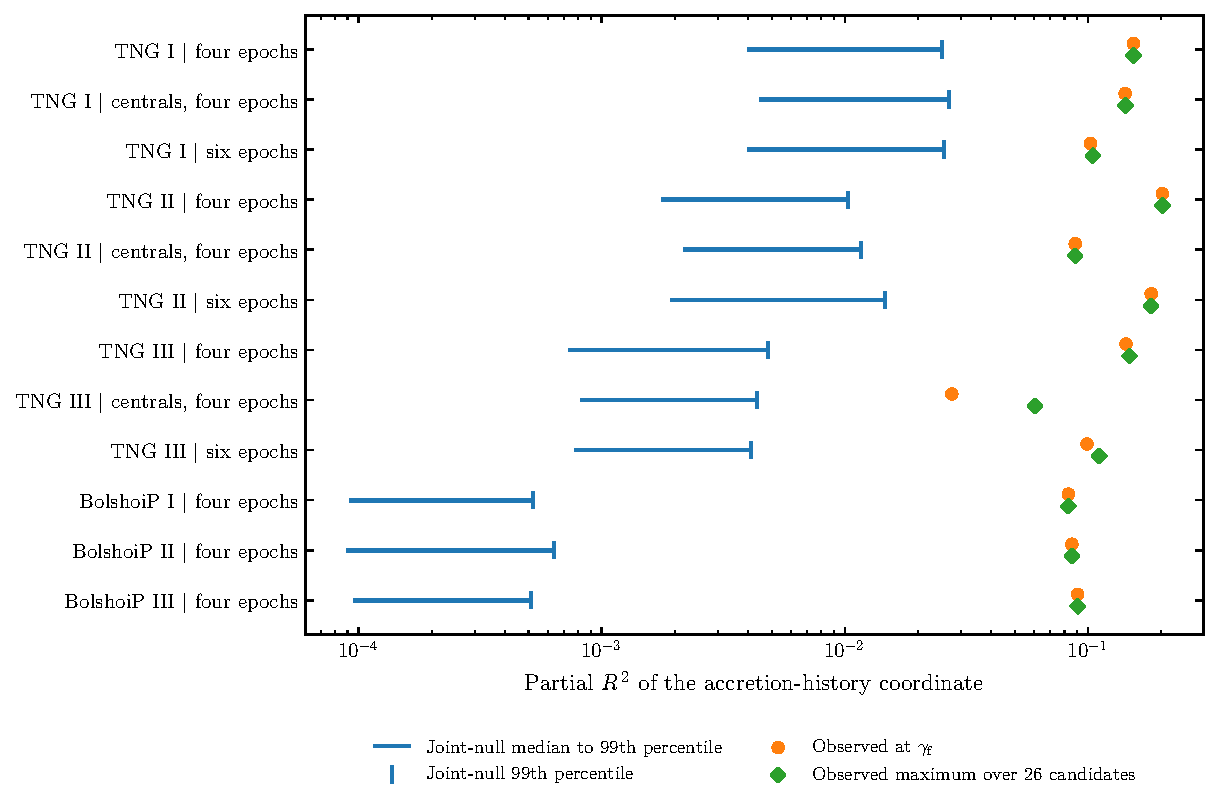
\includegraphics[width=.96\linewidth]{01_joint_search_null.pdf}
\caption{Observed partial $R^2$ at the fiducial parameter and at the best current candidate, compared with the median-to-99th-percentile range of the maximum-over-26 null statistic. The horizontal null summaries are not confidence intervals. Statistical dependence is discussed in Section~\ref{sec:limitations}.}\label{fig:joint}
\end{figure}

\subsection{Formation-epoch attenuation}
On matched rows, the four epochs attenuate the baseline-adjusted history increment by $75.2$--$82.7$ per cent in TNG and $84.4$--$84.9$ per cent in BolshoiP (Table~\ref{tab:matched}). The starting model already contains mass and current growth. BolshoiP omits approximately 21--22 per cent of available objects from the four-epoch fits; all 13,517 omissions lack an available $a_{10}$ crossing. The retained populations have higher mass, with standardized retained-minus-omitted log-mass differences of approximately $0.92$--$0.95$.
\begin{table}[htbp]\centering\small
\begin{tabular}{lrrrr}\toprule
Sample & $n_4$ & $\Delta R^2_{0}$ & $\Delta R^2_4$ & $f_{\rm att}$ \\\midrule
TNG I & 420 & 0.2458 & 0.0609 & 0.7521 \\
TNG II & 881 & 0.3199 & 0.0740 & 0.7687 \\
TNG III & 2,199 & 0.2750 & 0.0476 & 0.8268 \\
BolshoiP I & 16,126 & 0.2774 & 0.0432 & 0.8443 \\
BolshoiP II & 16,090 & 0.2879 & 0.0434 & 0.8492 \\
BolshoiP III & 16,340 & 0.2984 & 0.0453 & 0.8481 \\
\bottomrule\end{tabular}

\caption{Attenuation on the identical complete-case population for both history increments in each row. The values follow equation~\eqref{eq:att} and describe fitted variance increments, not causal fractions.}\label{tab:matched}
\end{table}

Adding $a_{05}$ and $a_{90}$ in TNG reduces the remaining increment by 42.9, 17.0 and 35.3 per cent in samples I--III. The comparisons use the same 419, 879 and 2,189 extended-complete objects for the four- and six-epoch fits. Six-epoch increments of $0.0354$, $0.0616$ and $0.0296$ remain, each with zero exceedances against its own full-search null (Table~\ref{tab:extended}). Adding both epochs together prevents attribution of the attenuation to $a_{05}$ alone. More flexible functions of these epochs and richer history summaries remain untested competitors.
\begin{table}[htbp]\centering\small
\begin{tabular}{llrrrr}\toprule
Sample & Epochs & $n$ & $\Delta R^2$ & $\Delta{\rm BIC}$ & $A\pm{\rm SE}$ \\\midrule
TNG I & Four & 419 & 0.0620 & $-64.94$ & $-0.314 \pm 0.036$ \\
TNG I & Six & 419 & 0.0354 & $-39.22$ & $-0.250 \pm 0.037$ \\
TNG II & Four & 879 & 0.0742 & $-192.01$ & $-0.373 \pm 0.025$ \\
TNG II & Six & 879 & 0.0616 & $-169.65$ & $-0.345 \pm 0.025$ \\
TNG III & Four & 2,189 & 0.0458 & $-316.90$ & $-0.277 \pm 0.015$ \\
TNG III & Six & 2,189 & 0.0296 & $-220.73$ & $-0.231 \pm 0.015$ \\
\bottomrule\end{tabular}

\caption{Four- and six-epoch comparisons on identical TNG populations. The six-epoch model adds $a_{05}$ and $a_{90}$. Conventional OLS errors are shown. Each six-epoch statistic attains $1/1001$ against its own 26-candidate rescan null.}\label{tab:extended}
\end{table}

\subsection{Dependence on the weighting parameter}
The six-point family $\{0.5,1.2,1.8,2.6,3.0,4.5\}$ gives negative coefficients in all 36 sample--parameter fits. For every cell, the candidate-specific comparison against its sample's saved minimum-over-26 null has zero exceedances. Table~\ref{tab:gamma} reports the effect ranges, amplitude maxima, BIC minima and candidate-specific full-search comparisons.
\begin{table}[htbp]\centering\footnotesize
\begin{tabular}{lrrccc}
\toprule
Sample & $\Delta R^2$ range & $A$ range & $\gamma_{\max|A|}$ & $\gamma_{\min\mathrm{BIC}}$ & Max. exceedances \\
\midrule
TNG I & 0.0283-$-0.0609$ & $-0.311$ to $-0.218$ & 1.8 & 1.8 & 0/1000 \\
TNG II & 0.0277-$-0.0740$ & $-0.373$ to $-0.244$ & 1.8 & 1.8 & 0/1000 \\
TNG III & 0.0204-$-0.0492$ & $-0.291$ to $-0.198$ & 1.8 & 2.6 & 0/1000 \\
BolshoiP I & 0.0173-$-0.0432$ & $-0.329$ to $-0.194$ & 1.2 & 1.2 & 0/1000 \\
BolshoiP II & 0.0168-$-0.0434$ & $-0.331$ to $-0.192$ & 1.2 & 1.2 & 0/1000 \\
BolshoiP III & 0.0198-$-0.0453$ & $-0.337$ to $-0.209$ & 1.2 & 1.2 & 0/1000 \\
\bottomrule
\end{tabular}

\caption{Six-point effect ranges and candidate-specific full-search comparisons. The last column is the largest exceedance count among that sample's six displayed values. $\gamma_{\max|A|}$ describes the six-point amplitude maximum; $\gamma_{\min\mathrm{BIC}}$ is the minimum over the full candidate family under the current controls. Ranges are descriptive, not uncertainty intervals.}\label{tab:gamma}
\end{table}

For mixed TNG III, the fiducial value is $3.0$. Under the final four-epoch controls, maximum $|A|$ occurs at $1.8$ but minimum BIC at $2.6$ ($D=-344.70$, compared with $-332.29$ at $3.0$). This is consistent with a change in the control model after the earlier selection. Neither criterion measures a physical relaxation timescale.

\section{Population dependence and numerical sensitivity}\label{sec:population}
\subsection{Current centrals and mixed TNG populations}
Removing satellites preserves a negative association in all three TNG samples but substantially changes its amplitude. At fixed $\gamma_{\rm f}$, the central-only increments are $0.0451$, $0.0266$ and $0.0078$, reductions of 26.0, 64.0 and 83.7 per cent relative to the mixed populations (Table~\ref{tab:central}). The corresponding native-slope magnitudes decrease by 19.1, 36.2 and 56.9 per cent. Each central-only fiducial-parameter statistic has zero joint-null exceedances.
\begin{table}[htbp]\centering\footnotesize
\begin{tabular}{lrrrrrrr}
\toprule
Sample & $n_c$ & $\gamma_{\rm f}$ & $A_c$ & $\Delta R^2_c$ & Drop (\%) & $\gamma_{\min\mathrm{BIC}}$ & $\Delta R^2_{c,\min\mathrm{BIC}}$ \\
\midrule
TNG I & 407 & 1.8 & $-0.2658$ & 0.0451 & 26.0 & 1.2 & 0.0453 \\
TNG II & 847 & 1.8 & $-0.2343$ & 0.0266 & 64.0 & 1.8 & 0.0266 \\
TNG III & 2,117 & 3.0 & $-0.1182$ & 0.0078 & 83.7 & 1.2 & 0.0171 \\
\bottomrule
\end{tabular}

\caption{Central-only four-epoch results. The drop compares $\Delta R^2$ with the mixed sample at the same fiducial parameter $\gamma_{\rm f}$. The last two columns separately describe the central-only BIC optimum and its increment; they do not replace $\gamma_{\rm f}$. The verified control ranks are $k_C=16,16,15$ for TNG I--III; the added history coefficient is separate.}\label{tab:central}
\end{table}

The excluded satellites constitute 3.7 per cent of TNG III. The reduction in the increment describes population sensitivity rather than an additive allocation of signal to satellites. Current central classification permits earlier environmental interactions.

The TNG III central-only BIC minimum occurs at $\gamma=1.2$, with $D=-124.84$ and $\Delta R^2=0.0171$, compared with $D=-51.44$ and $0.0078$ at the fiducial value $3.0$. Relative to the mixed fit at $3.0$, the optimized central increment is lower by approximately 64.0 per cent. This comparison changes both population and parameter rule. Even at each central sample's own BIC optimum, the increments span $0.0171$--$0.0453$; parameter choice only partly explains the within-TNG spread.

\begin{figure}[htbp]\centering
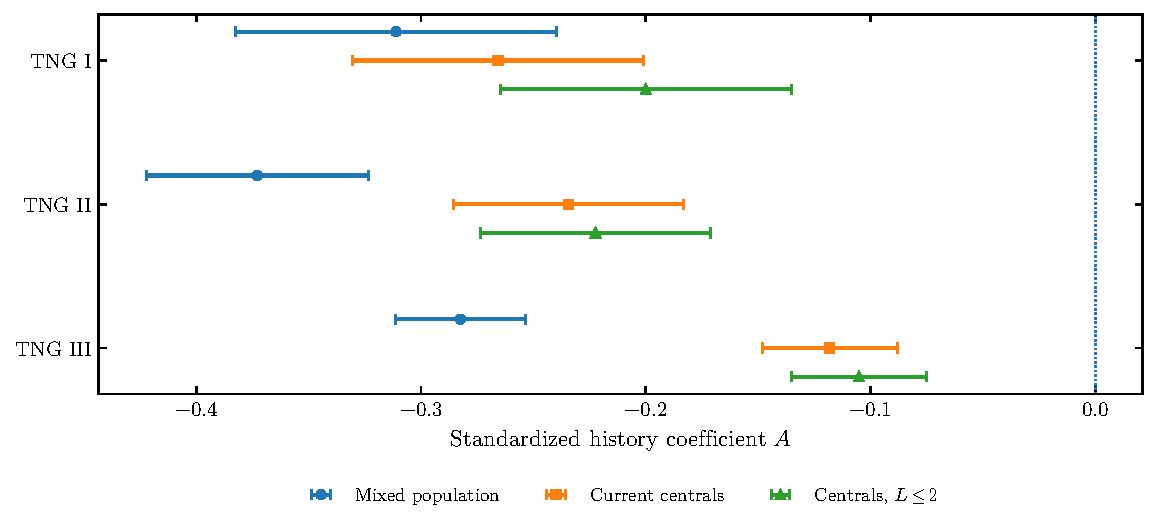
\includegraphics[width=\linewidth]{population_integrated.pdf}
\caption{TNG population sensitivity at unchanged $\gamma_{\rm f}$: mixed samples, current centrals, and centrals after excluding $L>2$. Bars are $1.96$ conventional OLS standard errors, with the qualifications in Section~\ref{sec:limitations}. Standardization is performed separately for each population. Native slopes are included in the machine-readable data described in Data Availability.}\label{fig:central}
\end{figure}

Among TNG centrals, $L>2$ holds for 5, 3 and 13 objects. Removing them leaves negative coefficients and increments of $0.0256$, $0.0241$ and $0.0061$ (Table~\ref{tab:tngloss}). The change is largest in relative terms for TNG I. The association is neither confined to current satellites nor to these large-recorded-loss centrals, but both population choices affect its amplitude.
\begin{table}[htbp]\centering\small
\begin{tabular}{lrrrrrr}
\toprule
Sample & Removed & $n$ & $A\pm\mathrm{SE}$ & $\Delta R^2$ & $\Delta\mathrm{BIC}$ & $b$ \\
\midrule
TNG I & 5 & 402 & $-0.1999\pm0.0331$ & 0.0256 & $-30.48$ & $-0.03408$ \\
TNG II & 3 & 844 & $-0.2224\pm0.0261$ & 0.0241 & $-64.21$ & $-0.03982$ \\
TNG III & 13 & 2,104 & $-0.1050\pm0.0153$ & 0.0061 & $-39.43$ & $-0.02959$ \\
\bottomrule
\end{tabular}

\caption{Additional descriptive TNG central-only fits with $L\leq2$, at the fiducial parameter. Counts removed are relative to the central sample. No new permutation probabilities are assigned to these three populations. Control ranks remain $k_C=16,16,15$ for TNG I--III, excluding the history coefficient.}\label{tab:tngloss}
\end{table}

\subsection{BolshoiP formation-threshold restrictions}
Both formation-threshold selections preserve negative coefficients at $\gamma_{\rm f}=1.2$ (Table~\ref{tab:threshold}). The $Q_{10}\geq20$ and $Q_{10}\geq50$ increments span $0.0509$--$0.0563$ and $0.0375$--$0.0524$, respectively, with zero exceedances in each sample's 1,000-draw full-search comparison.

\begin{table}[htbp]\centering\small
\begin{tabular}{llrrrrr}
\toprule
Sample & Selection & $n$ & $A\pm\mathrm{SE}$ & $\Delta R^2$ & $\Delta\mathrm{BIC}$ & $b$ \\
\midrule
BolshoiP I & Baseline & 16,126 & $-0.3288\pm0.0086$ & 0.0432 & $-1388.85$ & $-0.08530$ \\
BolshoiP I & $Q_{10}\geq20$ & 7,709 & $-0.4084\pm0.0123$ & 0.0509 & $-1021.85$ & $-0.09347$ \\
BolshoiP I & $Q_{10}\geq50$ & 3,423 & $-0.4069\pm0.0208$ & 0.0376 & $-356.33$ & $-0.08490$ \\
BolshoiP II & Baseline & 16,090 & $-0.3310\pm0.0085$ & 0.0434 & $-1433.78$ & $-0.08762$ \\
BolshoiP II & $Q_{10}\geq20$ & 7,699 & $-0.4240\pm0.0122$ & 0.0563 & $-1118.83$ & $-0.09728$ \\
BolshoiP II & $Q_{10}\geq50$ & 3,386 & $-0.4064\pm0.0199$ & 0.0375 & $-388.12$ & $-0.08619$ \\
BolshoiP III & Baseline & 16,340 & $-0.3365\pm0.0083$ & 0.0453 & $-1543.58$ & $-0.08698$ \\
BolshoiP III & $Q_{10}\geq20$ & 7,880 & $-0.4130\pm0.0119$ & 0.0520 & $-1111.91$ & $-0.09686$ \\
BolshoiP III & $Q_{10}\geq50$ & 3,455 & $-0.4730\pm0.0193$ & 0.0524 & $-549.41$ & $-0.09888$ \\
\bottomrule
\end{tabular}

\caption{BolshoiP threshold sensitivities at $\gamma_{\rm f}=1.2$. Errors are conventional OLS values; $b$ is the slope in catalogue units. Baseline and both cuts have zero of 1,000 joint-null exceedances. Each restricted null is generated on its own rows.}\label{tab:threshold}
\end{table}

Native-slope magnitudes increase by 9.6--11.4 per cent at $Q_{10}\geq20$; at 50 they range from 1.6 per cent smaller to 13.7 per cent larger than baseline. Of the 48,556 complete objects, 25,268 have $Q_{10}<20$; 12,997 of 13,517 missing crossings also lie below that value. Completeness therefore depends on mass scale without a universal 20-particle-equivalent cutoff. Bracketing-node masses and interpolation are described in Supplementary Material, Section~S2.

\subsection{Maximum-mass selection and recorded mass loss}\label{sec:loss}
Selection on $Q_{10}$ can retain objects whose terminal masses are substantially below their maxima. Objects with $L>2$ comprise approximately 1.1--2.1 per cent of the BolshoiP threshold-selected samples (Table~\ref{tab:losscount}).

\begin{table}[htbp]\centering\small
\begin{tabular}{lrrr}
\toprule
Sample & Baseline: $L>2$ & $Q_{10}\geq20$: $L>2$ & $Q_{10}\geq50$: $L>2$ \\
\midrule
BolshoiP I & 176/16,126 (1.09\%) & 130/7,709 (1.69\%) & 38/3,423 (1.11\%) \\
BolshoiP II & 200/16,090 (1.24\%) & 158/7,699 (2.05\%) & 43/3,386 (1.27\%) \\
BolshoiP III & 212/16,340 (1.30\%) & 165/7,880 (2.09\%) & 64/3,455 (1.85\%) \\
\bottomrule
\end{tabular}

\caption{Large recorded mass-loss counts among formation-complete BolshoiP populations. $L>2$ is a numerical history selection, not a classification of a particular stripping or orbital mechanism.}\label{tab:losscount}
\end{table}

Excluding this tail reduces the increments to $0.0348$--$0.0363$ at baseline, $0.0393$--$0.0436$ at $Q_{10}\geq20$ and $0.0279$--$0.0351$ at $Q_{10}\geq50$ (Table~\ref{tab:lossfits}; Fig.~\ref{fig:bp}). The negative association persists, with population-dependent amplitude. A terminal-mass selection, $Q_{10}^{\rm term}\geq20$, gives increments $0.0464$, $0.0485$ and $0.0507$. This changes only selection, not the formation-epoch definitions, and retains 36, 38 and 60 objects with $L>2$.

\begin{table}[htbp]\centering\small
\begin{tabular}{llrrrrr}
\toprule
Sample & Selection & $n$ & $k_C$ & $A$ & $\Delta R^2$ & $\Delta\mathrm{BIC}$ \\
\midrule
BolshoiP I & $L\leq2$ & 15,950 & 15 & $-0.3023$ & 0.0348 & $-1092.89$ \\
BolshoiP I & $Q_{10}\geq20,\ L\leq2$ & 7,579 & 15 & $-0.3662$ & 0.0393 & $-736.98$ \\
BolshoiP I & $Q_{10}\geq50,\ L\leq2$ & 3,385 & 14 & $-0.3623$ & 0.0279 & $-248.53$ \\
BolshoiP I & $Q_{10}^{\rm term}\geq20$ & 7,328 & 15 & $-0.3897$ & 0.0464 & $-831.69$ \\
BolshoiP II & $L\leq2$ & 15,890 & 15 & $-0.3093$ & 0.0359 & $-1162.97$ \\
BolshoiP II & $Q_{10}\geq20,\ L\leq2$ & 7,541 & 15 & $-0.3734$ & 0.0436 & $-813.01$ \\
BolshoiP II & $Q_{10}\geq50,\ L\leq2$ & 3,343 & 14 & $-0.3598$ & 0.0279 & $-267.58$ \\
BolshoiP II & $Q_{10}^{\rm term}\geq20$ & 7,284 & 15 & $-0.3900$ & 0.0485 & $-871.19$ \\
BolshoiP III & $L\leq2$ & 16,128 & 15 & $-0.3081$ & 0.0363 & $-1207.55$ \\
BolshoiP III & $Q_{10}\geq20,\ L\leq2$ & 7,715 & 15 & $-0.3685$ & 0.0406 & $-812.03$ \\
BolshoiP III & $Q_{10}\geq50,\ L\leq2$ & 3,391 & 14 & $-0.4003$ & 0.0351 & $-343.11$ \\
BolshoiP III & $Q_{10}^{\rm term}\geq20$ & 7,467 & 15 & $-0.3995$ & 0.0507 & $-974.67$ \\
\bottomrule
\end{tabular}

\caption{Descriptive BolshoiP mass-loss and terminal-selection refits, all at $\gamma_{\rm f}=1.2$. $k_C$ is the verified control rank. The terminal criterion changes selection, not the formation-control definition. No new permutation probabilities are attached to these 12 fixed-parameter fits.}\label{tab:lossfits}
\end{table}
\begin{figure}[htbp]\centering
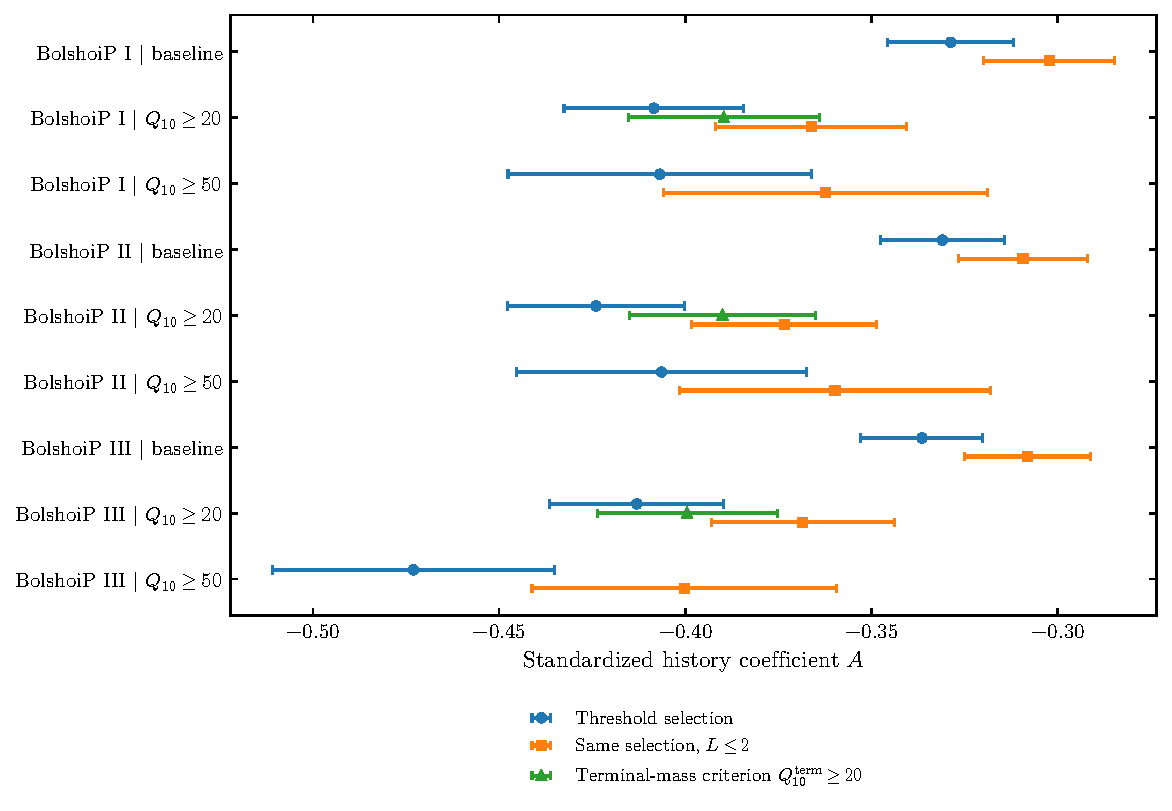
\includegraphics[width=.92\linewidth]{bp_population_integrated.pdf}
\caption{BolshoiP coefficients for baseline and maximum-mass-threshold populations, with and without the large-loss tail. Triangles at the $Q_{10}\geq20$ rows show the alternative terminal-mass selection. Bars denote conventional OLS uncertainty for each fit; the between-population differences have no separately estimated interval.}\label{fig:bp}
\end{figure}

All threshold-only designs have control rank 15. Combining $Q_{10}\geq50$ with $L\leq2$ empties the lowest native mass bin and reduces the rank to 14 (Supplementary Material, Section~S2). Current distinct-halo status and a mass ratio alone do not distinguish tidal processing, backsplash histories or catalogue effects.

\subsection{Comparison of central and distinct-halo populations}
At the fiducial parameters, the central-only TNG coefficients span $-0.266$ to $-0.118$, with increments $0.0078$--$0.0451$. BolshoiP distinct haloes give coefficients $-0.337$ to $-0.329$ and increments $0.0432$--$0.0453$. Both selections exclude current satellites; their different amplitudes and mass definitions remain explicit.

Applying $L\leq2$ to both populations leaves TNG increments $0.0061$--$0.0256$ and BolshoiP baseline increments $0.0348$--$0.0363$. The negative direction is shared, but a universal amplitude is unsupported. Bound central-subhalo mass and virial mass, sample mass distributions, history operators and formation completeness remain different even after the same numerical mass-loss exclusion. Current host status and $L\leq2$ also do not imply a common environmental history.


\subsection{Continuous recorded mass loss}\label{sec:continuous_loss}
Including $\ell$ on unchanged populations reduces the history contribution in every case (Table~\ref{tab:logloss}; Fig.~\ref{fig:logloss}). Mixed TNG increments fall to $0.0095$, $0.0089$ and $0.0035$ in samples I--III, reductions of 84.5, 88.0 and 92.7 per cent. 

The central-only increments become $0.0131$, $0.0124$ and $0.0023$, reductions of 71.0, 53.6 and 70.7 per cent relative to their own unaugmented controls. Because these comparisons use identical rows and response scales, the change is an overlap with the added historical summary rather than a change of population. 

\begin{table}[htbp]\centering\scriptsize
\setlength{\tabcolsep}{4pt}
\begin{tabular}{llrrrrr}\toprule
Sample & Population & $n$ & $A_{\ell}\pm\mathrm{SE}$ & $\Delta R^2_4$ & $\Delta R^2_{4,\ell}$ & $D_{\ell}$ \\ \midrule
TNG I & mixed & 420 & $-0.1322\pm0.0312$ & 0.0609 & 0.0095 & $-12.32$ \\
TNG II & mixed & 881 & $-0.1478\pm0.0241$ & 0.0740 & 0.0089 & $-30.84$ \\
TNG III & mixed & 2,199 & $-0.0865\pm0.0142$ & 0.0476 & 0.0035 & $-29.41$ \\
\addlinespace
TNG I & centrals & 407 & $-0.1567\pm0.0336$ & 0.0451 & 0.0131 & $-16.06$ \\
TNG II & centrals & 847 & $-0.1648\pm0.0251$ & 0.0266 & 0.0124 & $-36.16$ \\
TNG III & centrals & 2,117 & $-0.0655\pm0.0148$ & 0.0078 & 0.0023 & $-12.10$ \\
\addlinespace
BolshoiP I & baseline & 16,126 & $-0.2605\pm0.0100$ & 0.0432 & 0.0199 & $-656.23$ \\
BolshoiP II & baseline & 16,090 & $-0.2735\pm0.0101$ & 0.0434 & 0.0210 & $-709.53$ \\
BolshoiP III & baseline & 16,340 & $-0.2689\pm0.0099$ & 0.0453 & 0.0202 & $-705.88$ \\
\addlinespace
BolshoiP I & $Q_{10}\geq20$ & 7,709 & $-0.3052\pm0.0145$ & 0.0509 & 0.0200 & $-421.65$ \\
BolshoiP II & $Q_{10}\geq20$ & 7,699 & $-0.3276\pm0.0144$ & 0.0563 & 0.0236 & $-493.68$ \\
BolshoiP III & $Q_{10}\geq20$ & 7,880 & $-0.3149\pm0.0145$ & 0.0520 & 0.0200 & $-449.40$ \\
\addlinespace
BolshoiP I & $Q_{10}\geq50$ & 3,423 & $-0.2952\pm0.0249$ & 0.0376 & 0.0135 & $-130.20$ \\
BolshoiP II & $Q_{10}\geq50$ & 3,386 & $-0.2968\pm0.0235$ & 0.0375 & 0.0140 & $-148.80$ \\
BolshoiP III & $Q_{10}\geq50$ & 3,455 & $-0.3140\pm0.0243$ & 0.0524 & 0.0141 & $-156.03$ \\
\bottomrule\end{tabular}

\caption{Continuous recorded-loss control at fiducial $\gamma_{\rm f}$. $A_\ell$ and its conventional SE refer to the history coefficient after adding $\ell$, not to the coefficient of $\ell$. $\Delta R^2_4$ is the same-row four-epoch history increment and $\Delta R^2_{4,\ell}$ is the increment beyond four epochs and $\ell$. $D_\ell$ compares those latter nested models. These fiducial-parameter fits receive their own linear-design comparisons in Table~\ref{tab:loss_designs}. Native coefficients, the $\ell$ coefficient and covariance diagnostics are supplied at full precision.}\label{tab:logloss}
\end{table}

In BolshoiP, baseline increments become $0.0199$--$0.0210$, reductions of 51.6--55.5 per cent. The $Q_{10}\geq20$ increments become $0.0200$--$0.0236$, reductions of 58.1--61.5 per cent; the $Q_{10}\geq50$ increments become $0.0135$--$0.0141$, reductions of 62.6--73.1 per cent. 

All 15 adjusted history coefficients remain negative. The smallest additional BIC improvement is $D_\ell=-12.10$ in TNG III centrals. Conditional history--$\ell$ correlations range from approximately $-0.21$ to $-0.62$ after the earlier controls; the residual fraction of standardized $K$ variance after all controls is $0.14$--$0.54$. The remaining history direction is numerically identifiable. The nonlinear extension is assessed next.

\begin{figure}[htbp]\centering
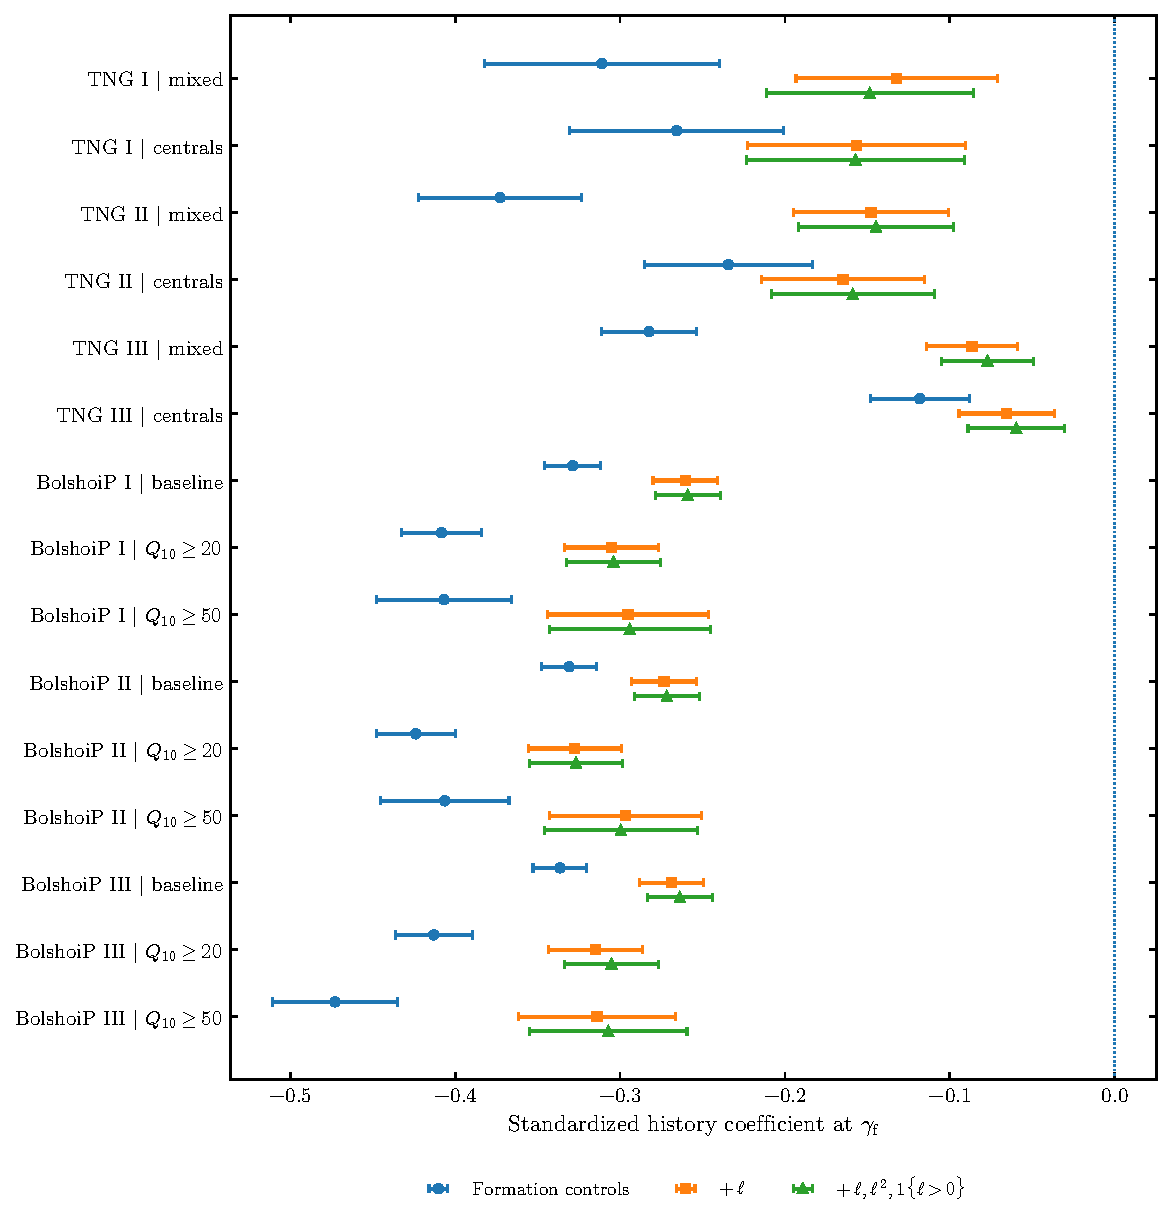
\includegraphics[width=.90\linewidth]{loss_control_comparison.pdf}
\caption{History coefficients under the formation-only, linear-loss and indicator-plus-quadratic control designs on the same objects and fiducial weighting parameter. Bars are $1.96$ conventional OLS standard errors, not uncertainty on coefficient differences or spatially adjusted intervals. Response and history scaling are identical within each population.}\label{fig:logloss}
\end{figure}

The TNG I central-only influence check helps interpret its five-object tail sensitivity. Before adding $\ell$, jointly excluding the five $L>2$ centrals changes the native history slope from $-0.04498$ to $-0.03408$, a 24.2 per cent decrease in magnitude. After adding $\ell$, the corresponding change is from $-0.02651$ to $-0.02680$, a 1.1 per cent increase. Thus the previously observed group-deletion change is largely accommodated by the linear recorded-loss summary in this sample. Other observations remain influential; no additional object is removed based on an influence statistic. Individual diagnostics and the singleton-bin case are given in Supplementary Material, Section~S3.

\subsection{Linear and flexible loss designs with their own search comparisons}\label{sec:loss_results}
The indicator and quadratic term do not systematically eliminate the post-linear residual (Table~\ref{tab:loss_designs}). Mixed TNG increments become $0.0112$, $0.0085$ and $0.0027$; central-only values become $0.0131$, $0.0113$ and $0.0018$. The baseline BolshoiP range is $0.0192$--$0.0205$, while the $Q_{10}\geq20$ and $Q_{10}\geq50$ ranges are $0.0186$--$0.0233$ and $0.0134$--$0.0141$. Adding nuisance terms need not decrease the incremental contribution of another regressor monotonically; TNG I mixed is an example. Every reported control matrix has full column rank, and each added history column increases rank by one.

\begin{table}[htbp]\centering\scriptsize\setlength{\tabcolsep}{3pt}
\begin{tabular}{llrrrrrr}
\toprule
Sample & Population & $\Delta R^2_\ell$ & $\Delta R^2_{\rm flex}$ & $D_{\rm flex}$ & $e_\ell$ & $e_{\rm flex}$ & $\gamma_{\min,\ell}/\gamma_{\min,\rm flex}$\\
\midrule
TNG I & mixed & 0.0095 & 0.0112 & $-15.90$ & 0 & 0 & 1.2/1.2\\
TNG I & centrals & 0.0131 & 0.0131 & $-16.17$ & 0 & 0 & 1.2/1.2\\
TNG II & mixed & 0.0089 & 0.0085 & $-29.81$ & 0 & 0 & 1.2/1.2\\
TNG II & centrals & 0.0124 & 0.0113 & $-33.01$ & 0 & 0 & 1.2/1.2\\
TNG III & mixed & 0.0035 & 0.0027 & $-21.71$ & 0 & 0 & 1.2/0.8\\
TNG III & centrals & 0.0023 & 0.0018 & $-8.46$ & 2 & 1 & 0.8/0.8\\
BolshoiP I & baseline & 0.0199 & 0.0195 & $-644.59$ & 0 & 0 & 0.8/0.5\\
BolshoiP I & $Q_{10}\geq20$ & 0.0200 & 0.0197 & $-416.61$ & 0 & 0 & 0.5/0.5\\
BolshoiP I & $Q_{10}\geq50$ & 0.0135 & 0.0134 & $-129.16$ & 0 & 0 & 0.5/0.5\\
BolshoiP II & baseline & 0.0210 & 0.0205 & $-694.34$ & 0 & 0 & 0.8/0.5\\
BolshoiP II & $Q_{10}\geq20$ & 0.0236 & 0.0233 & $-486.85$ & 0 & 0 & 0.5/0.3\\
BolshoiP II & $Q_{10}\geq50$ & 0.0140 & 0.0141 & $-149.28$ & 0 & 0 & 0.5/0.5\\
BolshoiP III & baseline & 0.0202 & 0.0192 & $-672.70$ & 0 & 0 & 0.8/0.5\\
BolshoiP III & $Q_{10}\geq20$ & 0.0200 & 0.0186 & $-418.37$ & 0 & 0 & 0.5/0.5\\
BolshoiP III & $Q_{10}\geq50$ & 0.0141 & 0.0134 & $-148.45$ & 0 & 0 & 0.5/0.5\\
\bottomrule
\end{tabular}

\caption{Same-population loss-design comparisons at fiducial $\gamma_{\rm f}$. $e$ counts null minima at least as favorable as the observed fiducial-parameter statistic, among 1,000 permutations per design. Thus $p=(e+1)/1001$. The last column gives descriptive full-grid BIC minima, not replacements for fiducial parameters. OLS estimates and search comparisons retain the qualifications in Section~\ref{sec:loss_search}.}\label{tab:loss_designs}
\end{table}

Twenty-eight of the 30 fiducial-parameter comparisons have no exceedance. TNG III centrals has two in the linear design and one in the flexible design, giving $3/1001$ and $2/1001$. Its corresponding $D$ values are $-12.10$ and $-8.46$. Holm adjustment across the 30 primary comparisons gives $0.02997$ for each. Single-step Bonferroni gives $0.02997$ for the zero-exceedance cases, but $0.08991$ and $0.05994$ for the two TNG III central cases. Those two do not reject at 0.05 under that single-step rule. All observed grid minima separately have zero exceedances. Treating primary and secondary comparisons together as a 60-member family gives Holm-adjusted values $0.05994$, hence no rejection at 0.05 at this Monte Carlo resolution. These statements use different comparison families and correction rules.

\subsection{Descriptive shift in BIC-preferred weighting}
After linear loss adjustment, BIC minima occur at $\gamma=0.8$--$1.2$ in TNG and $0.5$--$0.8$ in BolshoiP. With the indicator-plus-quadratic controls, the corresponding ranges are $0.8$--$1.2$ and $0.3$--$0.5$. All are below their fiducial values. For mixed TNG III, the linear-design minimum at $\gamma=1.2$ has $D\simeq-89.68$, compared with $-29.41$ at fiducial $\gamma=3.0$. Its full-grid minimum was already $2.6$ under the preceding four-epoch controls; different comparisons must therefore be distinguished. Some central-only four-epoch optima were already lower than the fiducial values, so loss adjustment does not newly shift every matched-population optimum.

Smaller $\gamma$ gives less rapidly declining weighting within each operator. These BIC optima describe the fitted historical representation; they do not measure a common physical relaxation time or out-of-sample accuracy.

\subsection{Restricted-cubic-spline sensitivity}\label{sec:spline}
The spline representation gives history increments of $0.0107$, $0.0086$ and $0.0028$ in mixed TNG, and $0.0130$, $0.0123$ and $0.0017$ among centrals. Across the nine BolshoiP populations, increments range from $0.0132$ to $0.0233$ (Table~\ref{tab:independent_spline}). Curvature represented by this spline therefore leaves a smaller residual correlation in both families.

\begin{table}[htbp]\centering\small
\begin{tabular}{llrrrr}
\toprule
Sample & Population & $\Delta R^2_{\rm spline}$ & $D_{\rm spline}$ & $e_{\ell,10k}$ & $e_{{\rm spline},10k}$\\
\midrule
TNG I & mixed & 0.0107 & $-14.83$ & 2 & 0\\
TNG I & centrals & 0.0130 & $-16.10$ & 2 & 1\\
TNG II & mixed & 0.0086 & $-29.74$ & 0 & 0\\
TNG II & centrals & 0.0123 & $-36.23$ & 0 & 0\\
TNG III & mixed & 0.0028 & $-22.83$ & 0 & 0\\
TNG III & centrals & 0.0017 & $-7.50$ & 0 & 3\\
BolshoiP I & baseline & 0.0193 & $-639.35$ & 0 & 0\\
BolshoiP I & $Q_{10}\geq20$ & 0.0197 & $-417.08$ & 0 & 0\\
BolshoiP I & $Q_{10}\geq50$ & 0.0132 & $-126.97$ & 0 & 0\\
BolshoiP II & baseline & 0.0203 & $-687.39$ & 0 & 0\\
BolshoiP II & $Q_{10}\geq20$ & 0.0233 & $-486.95$ & 0 & 0\\
BolshoiP II & $Q_{10}\geq50$ & 0.0141 & $-150.00$ & 0 & 0\\
BolshoiP III & baseline & 0.0190 & $-669.00$ & 0 & 0\\
BolshoiP III & $Q_{10}\geq20$ & 0.0188 & $-424.54$ & 0 & 0\\
BolshoiP III & $Q_{10}\geq50$ & 0.0137 & $-152.64$ & 0 & 0\\
\bottomrule
\end{tabular}

\caption{Restricted-cubic-spline sensitivity from the separately implemented calculations. The history coefficient uses the fiducial weighting parameter. Counts $e$ use 10,000 permutations per design and give $(e+1)/10001$. These are sample-specific, search-adjusted comparisons; they are not family-adjusted and are not pooled with the 1,000-draw results.}\label{tab:independent_spline}
\end{table}

For linear loss, the 10,000-draw calculations give two exceedances in TNG I mixed and central populations and zero in the other 13 populations. The spline calculations give one in TNG I centrals and three in TNG III centrals, with zero elsewhere. TNG III centrals is the weakest spline result, $\Delta R^2=0.0017$ and $D=-7.50$. These higher-budget calculations are reported as a separate numerical cross-check, rather than extending the primary resampling budget.

\subsection{Spatial and mass-distribution sensitivities}\label{sec:spatial_results}
All 945 delete-region fits retain a negative history coefficient across the nine populations, three control designs and two spatial grids. Under indicator-plus-quadratic loss controls, the TNG III central-only increments range from $0.0010$ to $0.0026$, compared with $0.0018$ in the full population; the corresponding BolshoiP ranges across the three baseline populations are $0.0169$--$0.0218$. The native-slope delete-region dispersion is $0.56$--$3.12$ times the conventional full-sample OLS standard error across all 54 design--grid combinations. These ratios describe geographic sensitivity rather than calibrated uncertainty inflation. Supplementary Table~S6 and Fig.~S4 summarize the flexible-loss fits; all design-specific results are provided in the numerical tables.

Using the mean-centred delete-region jackknife scale, coefficient-to-scale ratios are $4.33$--$15.21$ in TNG with formation controls alone and $2.10$--$4.22$ after linear or indicator-plus-quadratic loss adjustment. Across the three BolshoiP baseline populations, they are $9.75$--$37.70$ over all three control designs, and $9.75$--$22.86$ after loss adjustment. Nominal Student-$t$ references with $G-1$ degrees of freedom give the weakest two-sided values of $0.0455$ for mixed TNG I with linear loss on the 27-cell grid and $0.0468$ for TNG III centrals with flexible loss on the eight-cell grid. These pointwise fixed-parameter diagnostics do not adjust for the weighting-parameter search or multiple comparisons. Both grids and all 54 nominal intervals are reported in Supplementary Tables~S7--S8.

The three disjoint BolshoiP domains give similar native linear-loss-adjusted slopes, $-0.0676$, $-0.0724$ and $-0.0695$, with a between-domain sample standard deviation of $0.0024$. This is spatial consistency within one parent simulation rather than independent cosmological replication or evidence of exact amplitude equality. Supplementary Table~S9 reports the three control designs and an OLS-variance-based compatibility calculation with its assumptions stated explicitly.

Mass-bin reweighting preserves negative coefficients in all nine BolshoiP fits. The four-epoch increments change from $0.0432$--$0.0453$ to $0.0440$--$0.0461$, the linear-loss increments from $0.0199$--$0.0210$ to $0.0201$--$0.0209$, and the flexible-loss increments from $0.0192$--$0.0205$ to $0.0194$--$0.0203$. Native-slope magnitudes decrease by $0.3$--$1.2$ per cent. The retained-minus-available mean log-mass difference falls from $0.086$--$0.091$ dex to $0.021$--$0.022$ dex. Reweighting exactly matches the original bin frequencies, but residual within-bin mass differences remain (Supplementary Section~S6). These fits use observed complete cases only and have no additional inferential probabilities.

\section{Physical interpretation and limitations}
\subsection{Recorded mass loss and physical interpretation}
The dominant measured change is the substantial attenuation produced by continuous recorded-loss adjustment, especially in mixed TNG. Persistence under larger formation thresholds and continuous-loss attenuation answer different questions: the first restricts numerical coverage and mass population, while the second changes historical adjustment on identical rows. The threshold results disfavor an association confined to the lowest-threshold records without identifying measurement-error variance. Differential evolution of halo mass and inner velocity structure during tidal processing is a relevant physical interpretation. Controlled tidal-evolution calculations describe how subhalo density profiles and characteristic velocities change as material is removed \citep{Penarrubia2008,Errani2021,Benson2022}. This provides a physical precedent for mass-loss dependence, rather than establishing that our heterogeneous catalogue populations follow one tidal track. Current host classifications, maximum-to-terminal mass ratios and these regressions do not distinguish stripping from other dynamical or catalogue contributions.

The fitted coefficient of $\ell$ is not itself a calibrated stripping exponent. In an idealized track $V=V_0(M/M_0)^s$ with a fixed reference object, $Y_v$ changes with loss as $(1/3-s)\ell$. Across objects with $\log V_0=a+q\log M_0$, however,
\begin{equation}
Y_v=a+(q-1/3)\log M+(q-s)\ell.
\end{equation}
At fixed terminal mass, the coefficient is then $q-s$, equal to $1/3-s$ only after imposing $q=1/3$ and the other idealizations. The actual regression also conditions on formation epochs, current growth and the weighted history. We therefore report the positive native $\ell$ coefficients, approximately $0.160$--$0.213$ in TNG and $0.053$--$0.086$ in BolshoiP, without converting them into temporal tidal-track exponents.

A smaller accretion-history correlation remains under both loss designs and the spline sensitivity. The preference for less rapidly declining weighting after loss adjustment is compatible with the loss terms capturing part of the recent-growth association, but does not isolate a temporal channel. This limits the simple explanation that all of the original association is a consequence of the tested loss functions. It does not establish a new physical mechanism. Merger-driven structural responses \citep{Wang2020}, early-assembly relations \citep{Zhao2009}, and history--profile correspondence \citep{Ludlow2013,Ludlow2016} remain relevant interpretations or alternative historical compressions. The six-epoch test adds early and late thresholds together and cannot identify their separate contributions.

\subsection{Scope of inference}\label{sec:limitations}
The effects are conditional, in-sample regression associations. The regression figures use conventional OLS covariance; Supplementary Tables~S7--S8 separately give nominal jackknife-based Student-$t$ intervals. These nominal references are pointwise and hold the data-informed weighting parameter fixed. They require additional cross-region and finite-cluster assumptions, and do not combine with the permutation comparisons to form one spatially calibrated, search-adjusted test. Global residual permutations require exchangeability that has not been established for spatially correlated haloes. The spatial deletion results quantify dependence on the chosen regions; unequal occupancy, correlations across cell boundaries and modes larger than the sampled volume prevent treating their dispersion as a validated sampling error. The samples share simulation volumes, and several sensitivity populations overlap; they are not independent cosmological realizations. Search adjustment covers the stated 26-value family and the specified comparison families, not every earlier analytical choice.

The formation-complete BolshoiP relation is conditional on available crossings. The 13,517 omitted crossings precede the first sampled point, and the retained population is more massive. Mass-bin reweighting addresses the measured change in stratum frequencies only. Neither the missing epochs nor the direction of any full-population coefficient bias is identified without additional assumptions about the unobserved histories. Higher mass-equivalent thresholds argue against an association confined to the least-resolved histories, but they also change the mass distribution. Correlated errors in formation epochs and $K_\gamma$, tree interpolation and finite sampling remain possible. Direct TNG counts and timestep diagnostics characterize one resolution and do not establish convergence.

Population exclusions and added controls answer different questions. Changes in fitted increments are neither causal allocations to excluded objects nor information-theoretic decompositions. Linear, quadratic and spline loss terms test particular functions; richer loss or formation-history representations could explain additional variation. A negative history coefficient is not a physical damping parameter, and a small nonzero increment does not establish useful out-of-sample accuracy or a non-Markovian equation of motion.

\subsection{Prospective dynamical and observational tests}
The results motivate a non-Markovian cosmological modelling question: whether an explicit historical response improves future evolution after conditioning on a sufficiently informative present state, and whether that response can be represented by a compact, recursively updateable state. Such a test needs fixed forecast origins, independent evaluation roles, time-ordered histories and strong present-state competitors. An adequate augmented state is a meaningful outcome even if finer residual associations remain detectable.

Observational reconstruction would additionally require a generative link from histories to observable quantities, together with uncertainty propagation and selection modelling. Neither clustering nor lensing consequences are measured here. The structural correlations studied here motivate these prospective dynamical and observational tests.

\section{Conclusions}
A weighted accretion-history coordinate adds structural association beyond the specified mass, current-growth and four formation-epoch controls. Joint weighting-parameter permutation tests quantify that association under their stated resampling model. Central-only, formation-threshold and large-recorded-loss restrictions show that its amplitude depends on population.

The continuous historical summary $\ell=\log_{10}(\Mrec/\Mterm)$ explains an additional, substantial part of the fitted increment: the reductions are 84.5--92.7 per cent in mixed TNG samples, 53.6--71.0 per cent among TNG centrals and 51.6--73.1 per cent across the BolshoiP populations. A smaller negative history coefficient remains under both loss designs in all 15 populations, with design-specific search comparisons and the multiplicity qualifications reported above. The principal conclusion is substantial mass-loss dependence of the fitted structural correlation, with a smaller population-dependent association remaining beyond the specified formation epochs and tested loss functions. It is not an identified dynamical memory law. Future predictive-closure work must assess whether a compact, evolving historical state achieves adequate forecasts on independently evaluated data.

\section*{Acknowledgements}
This work uses the IllustrisTNG and Bolshoi--Planck simulations and the associated halo-catalogue and merger-tree products. The TNG100/300 presentation series comprises \citet{Pillepich2018,Springel2018,Nelson2018,Naiman2018,Marinacci2018}, together with the public release \citep{Nelson2019}. The author acknowledges the teams responsible for these data and numerical methods. ChatGPT (OpenAI) and Claude (Anthropic) were used at the author's direction for code development, numerical checking and manuscript editing. Claude was used to write the second fitting and spline implementation without reading or importing the analysis fitting functions. AI-assisted checks included direct OLS comparisons, algebraic identities and seeded numerical reproduction. The author is responsible for the analysis, interpretation and final text.


The CosmoSim database used in this paper is a service by the Leibniz-Institute for Astrophysics Potsdam (AIP). The MultiDark database was developed in cooperation with the Spanish MultiDark Consolider Project CSD2009-00064.

The author gratefully acknowledges the Gauss Centre for Supercomputing e.V. (\url{www.gauss-centre.eu}) and the Partnership for Advanced Supercomputing in Europe (PRACE, \url{www.prace-ri.eu}) for funding the MultiDark simulation project by providing computing time on the GCS Supercomputer SuperMUC at Leibniz Supercomputing Centre (LRZ, \url{www.lrz.de}). The Bolshoi simulations have been performed within the Bolshoi project of the University of California High-Performance AstroComputing Center (UC-HiPACC) and were run at the NASA Ames Research Center.



\section*{Data availability}
\AnalysisAvailability{} IllustrisTNG catalogues and merger trees are available through the project data service \citep{Nelson2019,TNGSpec}; BolshoiP catalogues and trees are distributed through the simulation data services and CosmoSim schema \doi{10.17876/cosmosim/bolshoip} \citep{CosmoBolshoiP}. Access to upstream simulation products follows the providers' conditions.

{\small\setlength{\bibsep}{1.5pt}\interlinepenalty=10000\begin{thebibliography}{99}
\bibitem[Behroozi et al.(2013a)]{Behroozi2013a}
Behroozi P. S., Wechsler R. H., Wu H.-Y., 2013a, ApJ, 762, 109. The ROCKSTAR phase-space temporal halo finder and the velocity offsets of cluster cores. \doi{10.1088/0004-637X/762/2/109}

\bibitem[Behroozi et al.(2013b)]{Behroozi2013b}
Behroozi P. S., Wechsler R. H., Wu H.-Y., Busha M. T., Klypin A. A., Primack J. R., 2013b, ApJ, 763, 18. Gravitationally consistent halo catalogs and merger trees for precision cosmology. \doi{10.1088/0004-637X/763/1/18}

\bibitem[Benson \& Du(2022)]{Benson2022}
Benson A. J., Du X., 2022, MNRAS, 517, 1398. Tidal tracks and artificial disruption of cold dark matter halos. \doi{10.1093/mnras/stac2750}

\bibitem[Bullock et al.(2001)]{Bullock2001}
Bullock J. S., Kolatt T. S., Sigad Y., Somerville R. S., Kravtsov A. V., Klypin A. A., Primack J. R., Dekel A., 2001, MNRAS, 321, 559--575. Profiles of dark haloes: evolution, scatter and environment. \doi{10.1046/j.1365-8711.2001.04068.x}

\bibitem[Cameron \& Miller(2015)]{CameronMiller2015}
Cameron A. C., Miller D. L., 2015, Journal of Human Resources, 50, 317--372. A practitioner's guide to cluster-robust inference. \doi{10.3368/jhr.50.2.317}

\bibitem[CosmoSim(2026a)]{CosmoSpec}
CosmoSim, 2026a, BolshoiP ROCKSTAR catalogue specification. \url{https://www.cosmosim.org/metadata/bolshoip/rockstar/}. Dataset identifier: \doi{10.17876/cosmosim/bolshoip/009}

\bibitem[CosmoSim(2026b)]{CosmoBolshoiP} CosmoSim. 2026b, BolshoiP database schema, Leibniz Institute for Astrophysics Potsdam. \doi{10.17876/cosmosim/bolshoip}. 

\bibitem[Diemer(2023)]{Diemer2023}
Diemer B., 2023, MNRAS, 519, 3292--3311. A dynamics-based density profile for dark haloes---II. Fitting function. \doi{10.1093/mnras/stac3778}

\bibitem[Diemer \& Joyce(2019)]{DiemerJoyce2019}
Diemer B., Joyce M., 2019, ApJ, 871, 168. An accurate physical model for halo concentrations. \doi{10.3847/1538-4357/aafad6}

\bibitem[Errani \& Navarro(2021)]{Errani2021}
Errani R., Navarro J. F., 2021, MNRAS, 505, 18--32. The asymptotic tidal remnants of cold dark matter subhaloes. \doi{10.1093/mnras/stab1215}

\bibitem[IllustrisTNG(2026a)]{TNGSpec}
IllustrisTNG, 2026a, Public data specifications. \url{https://www.tng-project.org/data/docs/specifications/}

\bibitem[IllustrisTNG(2026b)]{TNGDownload}
IllustrisTNG, 2026b, TNG100-1-Dark data and simulation metadata. \url{https://www.tng-project.org/data/downloads/TNG100-1-Dark/}.

\bibitem[IllustrisTNG(2026c)]{TNGAPI}
IllustrisTNG, 2026c, Public API documentation: subhalo identity and primary flag. \url{https://www.tng-project.org/data/docs/api/}.

\bibitem[Klypin et al.(2016)]{Klypin2016}
Klypin A., Yepes G., Gottl\"ober S., Prada F., He\ss{} S., 2016, MNRAS, 457, 4340--4359. MultiDark simulations: the story of dark matter halo concentrations and density profiles. \doi{10.1093/mnras/stw248}

\bibitem[Lucie-Smith et al.(2022)]{LS2022}
Lucie-Smith L., Adhikari S., Wechsler R. H., 2022, MNRAS, 515, 2164--2177. Insights into the origin of halo mass profiles from machine learning. \doi{10.1093/mnras/stac1833}

\bibitem[Lucie-Smith et al.(2024)]{LS2024}
Lucie-Smith L., Peiris H. V., Pontzen A., 2024, Phys. Rev. Lett., 132, 031001. Explaining dark matter halo density profiles with neural networks. \doi{10.1103/PhysRevLett.132.031001}

\bibitem[Ludlow et al.(2013)]{Ludlow2013}
Ludlow A. D., Navarro J. F., Boylan-Kolchin M., Bett P. E., Angulo R. E., Li M., White S. D. M., Frenk C., Springel V., 2013, MNRAS, 432, 1103--1113. The mass profile and accretion history of cold dark matter haloes. \doi{10.1093/mnras/stt526}

\bibitem[Ludlow et al.(2016)]{Ludlow2016}
Ludlow A. D., Bose S., Angulo R. E., Wang L., Hellwing W. A., Navarro J. F., Cole S., Frenk C. S., 2016, MNRAS, 460, 1214--1232. The mass--concentration--redshift relation of cold and warm dark matter haloes. \doi{10.1093/mnras/stw1046}

\bibitem[MacKinnon et al.(2023)]{MacKinnon2023}
MacKinnon J. G., Nielsen M. {\O}., Webb M. D., 2023, Journal of Applied Econometrics, 38, 671--694. Fast and reliable jackknife and bootstrap methods for cluster-robust inference. \doi{10.1002/jae.2969}

\bibitem[Marinacci et al.(2018)]{Marinacci2018}
Marinacci F., et al., 2018, MNRAS, 480, 5113--5139. First results from the IllustrisTNG simulations: radio haloes and magnetic fields. \doi{10.1093/mnras/sty2206}

\bibitem[Naiman et al.(2018)]{Naiman2018}
Naiman J. P., et al., 2018, MNRAS, 477, 1206--1224. First results from the IllustrisTNG simulations: a tale of two elements---chemical evolution of magnesium and europium. \doi{10.1093/mnras/sty618}

\bibitem[Navarro et al.(1997)]{NFW1997}
Navarro J. F., Frenk C. S., White S. D. M., 1997, ApJ, 490, 493--508. A universal density profile from hierarchical clustering. \doi{10.1086/304888}

\bibitem[Nelson et al.(2018)]{Nelson2018}
Nelson D., et al., 2018, MNRAS, 475, 624--647. First results from the IllustrisTNG simulations: the galaxy colour bimodality. \doi{10.1093/mnras/stx3040}

\bibitem[Nelson et al.(2019)]{Nelson2019}
Nelson D., et al., 2019, Computational Astrophysics and Cosmology, 6, 2. The IllustrisTNG simulations: public data release. \doi{10.1186/s40668-019-0028-x}

\bibitem[Norberg et al.(2009)]{Norberg2009}
Norberg P., Baugh C. M., Gazta\~naga E., Croton D. J., 2009, MNRAS, 396, 19--38. Statistical analysis of galaxy surveys---I. Robust error estimation for two-point clustering statistics. \doi{10.1111/j.1365-2966.2009.14389.x}

\bibitem[Pe\~narrubia et al.(2008)]{Penarrubia2008}
Pe\~narrubia J., Navarro J. F., McConnachie A. W., 2008, ApJ, 673, 226. The tidal evolution of Local Group dwarf spheroidals. \doi{10.1086/523686}

\bibitem[Pillepich et al.(2018)]{Pillepich2018}
Pillepich A., et al., 2018, MNRAS, 475, 648--675. First results from the IllustrisTNG simulations: the stellar mass content of groups and clusters of galaxies. \doi{10.1093/mnras/stx3112}

\bibitem[Rodriguez-Gomez et al.(2015)]{RG2015}
Rodriguez-Gomez V., et al., 2015, MNRAS, 449, 49--64. The merger rate of galaxies in the Illustris simulation: a comparison with observations and semi-empirical models. \doi{10.1093/mnras/stv264}

\bibitem[Rodr\'{i}guez-Puebla et al.(2016)]{RodriguezPuebla2016}
Rodr\'{i}guez-Puebla A., et al., 2016, MNRAS, 462, 893--916. Halo and subhalo demographics with Planck cosmological parameters: Bolshoi--Planck and MultiDark--Planck simulations. \doi{10.1093/mnras/stw1705}

\bibitem[Springel et al.(2001)]{Springel2001}
Springel V., White S. D. M., Tormen G., Kauffmann G., 2001, MNRAS, 328, 726--750. Populating a cluster of galaxies---I. Results at $z=0$. \doi{10.1046/j.1365-8711.2001.04912.x}

\bibitem[Springel et al.(2018)]{Springel2018}
Springel V., et al., 2018, MNRAS, 475, 676--698. First results from the IllustrisTNG simulations: matter and galaxy clustering. \doi{10.1093/mnras/stx3304}

\bibitem[Theoretical Astrophysical Observatory(2026)]{TAO}
Theoretical Astrophysical Observatory, 2026, Bolshoi (Planck) data guide: simulation parameters and mass resolution. \url{https://tao.asvo.org.au/tao/static/documentation/sim-bolshoi-planck.html}.

\bibitem[Wang et al.(2020)]{Wang2020}
Wang K., Mao Y.-Y., Zentner A. R., Lange J. U., van den Bosch F. C., Wechsler R. H., 2020, MNRAS, 498, 4450--4464. Concentrations of dark haloes emerge from their merger histories. \doi{10.1093/mnras/staa2733}

\bibitem[Wechsler et al.(2002)]{Wechsler2002}
Wechsler R. H., Bullock J. S., Primack J. R., Kravtsov A. V., Dekel A., 2002, ApJ, 568, 52--70. Concentrations of dark halos from their assembly histories. \doi{10.1086/338765}

\bibitem[Winkler et al.(2014)]{Winkler2014}
Winkler A. M., Ridgway G. R., Webster M. A., Smith S. M., Nichols T. E., 2014, NeuroImage, 92, 381--397. Permutation inference for the general linear model. \doi{10.1016/j.neuroimage.2014.01.060}

\bibitem[Wong \& Taylor(2012)]{Wong2012}
Wong A. W. C., Taylor J. E., 2012, ApJ, 757, 102. What do dark matter properties tell us about their mass assembly histories? \doi{10.1088/0004-637X/757/1/102}

\bibitem[Zhao et al.(2009)]{Zhao2009}
Zhao D. H., Jing Y. P., Mo H. J., B\"orner G., 2009, ApJ, 707, 354--369. Accurate universal models for the mass accretion histories and concentrations of dark matter halos. \doi{10.1088/0004-637X/707/1/354}

\end{thebibliography}
}
\end{document}
